\documentclass[12pt]{article}
\usepackage{amsmath}
\usepackage{graphicx}
\usepackage{hyperref}
\usepackage{listings}
\usepackage{color}
\usepackage{pythonhighlight}
\usepackage{indentfirst}

\title{Operating System Course Report - First Half of the Semester}
\author{A class}
\date{\today}

\begin{document}

\maketitle
\newpage

\tableofcontents
\newpage

\section{Introduction}
This report summarizes the topics covered during the first half of the Operating System course. It includes theoretical concepts, practical implementations, and assignments. The course focuses on the fundamentals of operating systems, including system architecture, process management, CPU scheduling, and deadlock handling.

\section{Course Overview}
\subsection{Objectives}
The main objectives of this course are:
\begin{itemize}
    \item To understand the basic components and architecture of a computer system.
    \item To learn process management, scheduling, and inter-process communication.
    \item To explore file systems, input/output management, and virtualization.
    \item To study the prevention and handling of deadlocks in operating systems.
\end{itemize}

\subsection{Course Structure}
The course is divided into two halves. This report focuses on the first half, which covers:
\begin{itemize}
    \item Basic Concepts and Components of Computer Systems
    \item System Performance and Metrics
    \item System Architecture of Computer Systems
    \item Process Description and Control
    \item Scheduling Algorithms
    \item Process Creation and Termination
    \item Introduction to Threads
    \item File Systems
    \item Input and Output Management
    \item Deadlock Introduction and Prevention
    \item User Interface Management
    \item Virtualization in Operating Systems
\end{itemize}

\section{Topics Covered}

\subsection{Basic Concepts and Components of Computer Systems}
This section explains the fundamental components that make up a computer system, including the CPU, memory, storage, and input/output devices.

\subsection{System Performance and Metrics}
This section introduces various system performance metrics used to measure the efficiency of a computer system, including throughput, response time, and utilization.

\subsection{System Architecture of Computer Systems}
Describes the architecture of modern computer systems, focusing on the interaction between hardware and the operating system.

\subsection{Process Description and Control}
Processes are a central concept in operating systems. This section covers:
\begin{itemize}
    \item Process states and state transitions
    \item Process control block (PCB)
    \item Context switching
\end{itemize}

\subsection{Scheduling Algorithms}
This section covers:
\begin{itemize}
    \item First-Come, First-Served (FCFS)
    \item Shortest Job Next (SJN)
    \item Round Robin (RR)
\end{itemize}
It explains how these algorithms are used to allocate CPU time to processes.

\subsection{Process Creation and Termination}
Details how processes are created and terminated by the operating system, including:
\begin{itemize}
    \item Process spawning
    \item Process termination conditions
\end{itemize}

\subsection{Introduction to Threads}
\subsubsection{Konsep Threads}

% Materi Restu Ahmadinata - H071231021

\subsubsection{Hubungan antara Proses dan \textit{Threads}}

\textit{Threads} dan proses memiliki hubungan yang sangat erat dalam mengeksekusi program di dalam komputer. \textbf{Proses} merupakan unit eksekusi mandiri yang berjalan dengan memiliki ruang memori, sumber daya, dan lingkungan eksekusi yang terisolasi dari proses-proses lain. Sebuah proses dapat menjalankan program secara independen dan memanfaatkan memori serta sumber daya yang dialokasikan oleh sistem operasi. Di dalam sebuah proses, bisa terdapat satu atau lebih \textit{threads}. \textbf{\textit{Thread}} adalah unit eksekusi yang lebih kecil dan lebih ringan dibanding dengan proses. 

\hspace{1cm}

\textit{Thread} berbagi ruang memori dan sumber daya yang sama dengan proses induknya, namun setiap \textit{thread} memiliki \textit{stack} dan \textit{register} tersendiri. Hal tersebut memungkinkan beberapa \textit{threads} menjalankan tugas-tugas berbeda secara paralel, namun tetap terkoordinasi dalam satu proses yang sama. Karena \textit{threads} berbagi sumber daya yang sama dengan proses induk, eksekusi \textit{thread} jauh lebih ringan dibanding jika harus membuat proses baru. Maka dari itulah, \textit{threads} sering digunakan untuk meningkatkan efisiensi dan performa, terutama dalam aplikasi yang memerlukan banyak tugas dilakukan secara bersamaan.

\hspace{1cm}

Salah satu aplikasi desain grafis yaitu Canva dapat dijadikan sebagai contoh untuk menjelaskan hubungan antara \textit{threads} dan proses. Ketika pengguna membuka aplikasi Canva, berikut adalah bagaimana proses dan \textit{threads} berkolaborasi:

\begin{enumerate}
    \item \textbf{Proses Canva:} Ketika pengguna menjalankan aplikasi Canva, sistem operasi akan membuat sebuah proses baru. Proses ini mencakup semua sumber daya yang dibutuhkan oleh aplikasi untuk berjalan dengan baik, termasuk memori, \textit{CPU time}, dan file pendukung. Proses ini juga akan mengelola seluruh komponen aplikasi, mulai dari antarmuka pengguna hingga alat desain yang tersedia.
    
    \item \textbf{\textit{Threads} di dalam Proses Canva:} Aplikasi Canva memanfaatkan \textit{multithreading} untuk menangani beberapa tugas secara bersamaan tanpa harus membuat proses baru. Berikut adalah beberapa contoh \textit{thread} yang bekerja di dalam proses Canva:
    
    \begin{itemize}
        \item \textbf{\textit{Thread} 1: Antarmuka Pengguna (UI) -} \textit{Thread} ini bertanggung jawab untuk menampilkan dan menjaga responsivitas elemen-elemen visual seperti tombol, menu, dan panel desain di Canva. \textit{Thread} ini memastikan bahwa pengguna dapat berinteraksi dengan antarmuka secara lancar.
        \item \textbf{\textit{Thread} 2: Pemrosesan Gambar -} Ketika pengguna mengunggah, mengedit, atau menambahkan filter pada gambar atau elemen grafis, \textit{thread} ini akan menangani pemrosesan tersebut secara paralel, sehingga Canva tetap bisa berjalan tanpa mengalami penurunan performa.
        \item \textbf{\textit{Thread} 3: Sinkronisasi dengan \textit{Server} -} \textit{Thread} ini berfungsi untuk menyimpan hasil desain secara otomatis di \textit{cloud} Canva dan memastikan desain yang dikerjakan pengguna selalu diperbarui. Proses ini dilakukan di latar belakang tanpa mengganggu aktivitas utama pengguna.
    \end{itemize}

    % Ilustrasi
    \begin{figure}[h]
        \centering
        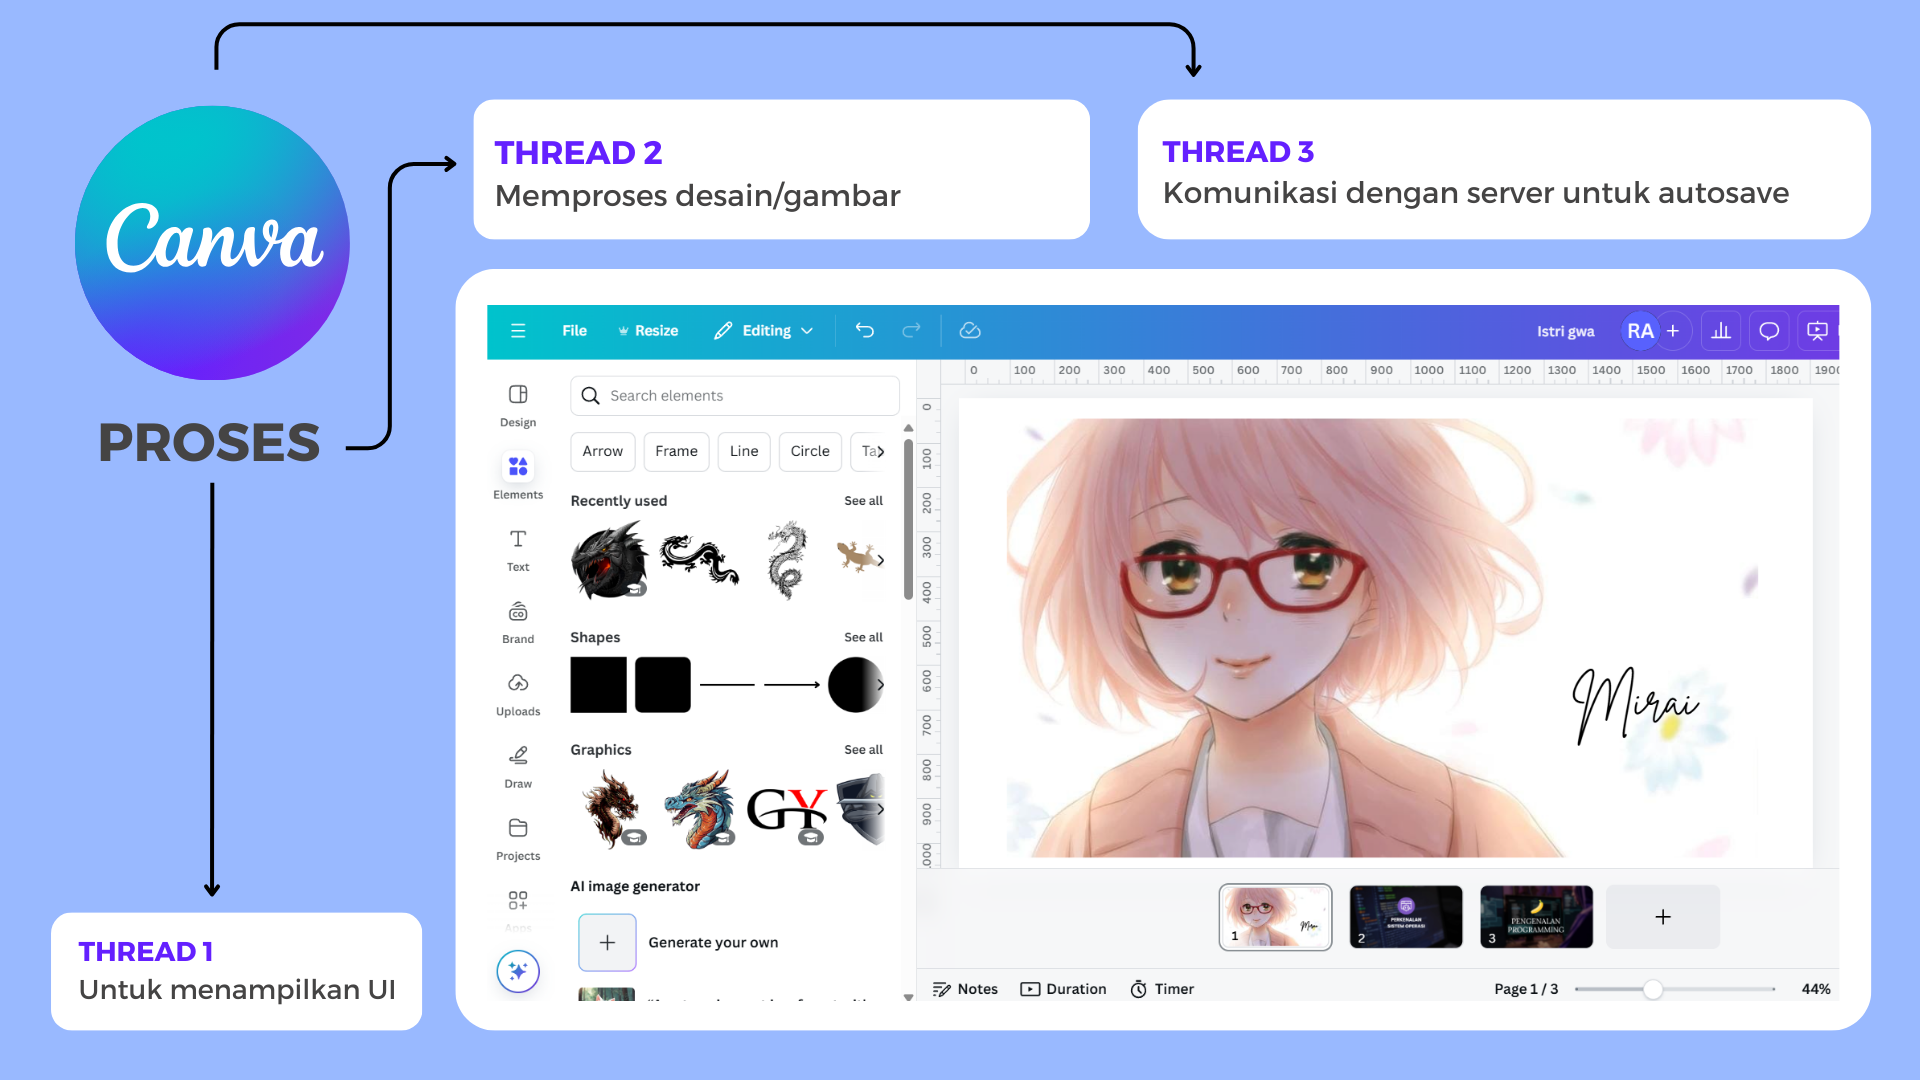
\includegraphics[width=1\linewidth]{asset/process-and-threads-illustration.png}
        \caption{Ilustrasi hubungan proses dan \textit{threads}}
        \label{fig:ilustrasi-proses-dan-threads}
    \end{figure}
    
\end{enumerate}

\hspace{1cm}

Hubungan antara \textit{threads} dan proses dalam sebuah aplikasi penting untuk menjaga efisiensi dan performa aplikasi tersebut. \textit{Threads} memungkinkan berbagai tugas dapat dilakukan secara bersamaan dalam satu proses yang sama. Hal tersebut dapat mengurangi \textit{overhead} yang dihasilkan jika setiap tugas dijalankan dalam proses yang berbeda. Dengan demikian, \textit{threads} memberikan pengalaman yang lebih responsif dan efisien bagi pengguna, karena setiap \textit{thread} dapat fokus pada tugas spesifik, namun tetap berbagi sumber daya yang sama dalam proses induknya.

% END OF THE LINE
\hspace{1cm}
\hline
\hspace{1cm}

\begin{figure}[h]
    \centering
    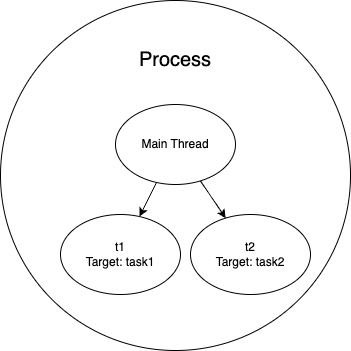
\includegraphics[width=0.5\textwidth]{/Users/khawaritzmi/Unhas/os_report_mid2024/a_class/asset/example.png}  % Sesuaikan nama file dan ukurannya
    \caption{Ini adalah gambar contoh dari multithreading.}
    \label{fig:contoh_gambar}
\end{figure}

Seperti yang terlihat pada Gambar \ref{fig:contoh_gambar}, inilah cara menambahkan gambar dengan keterangan.

\subsection{File Systems}
File systems provide a way for the operating system to store, retrieve, and manage data. This section explains:
\begin{itemize}
    \item File system structure
    \item File access methods
    \item Directory management
\end{itemize}

\subsection{Input and Output Management}
Input and output management is key for handling the interaction between the system and external devices. This section includes:
\begin{itemize}
    \item Device drivers
    \item I/O scheduling
\end{itemize}

\subsection{Deadlock Introduction and Prevention}
Explores the concept of deadlocks and methods for preventing them:
\begin{itemize}
    \item Deadlock conditions
    \item Deadlock prevention techniques
\end{itemize}

\subsection{User Interface Management}
This section discusses the role of the operating system in managing the user interface. Topics covered include:
\begin{itemize}
    \item Graphical User Interface (GUI)
    \item Command-Line Interface (CLI)
    \item Interaction between the user and the operating system
\end{itemize}

\subsection{Virtualization in Operating Systems}
Virtualization allows multiple operating systems to run concurrently on a single physical machine. This section explores:
\begin{itemize}
    \item Concept of virtualization
    \item Hypervisors and their types
    \item Benefits of virtualization in modern computing
\end{itemize}

\section{Assignments and Practical Work}
\subsection{Assignment 1: Process Scheduling}
Students were tasked with implementing various process scheduling algorithms (e.g., FCFS, SJN, and RR) and comparing their performance under different conditions.
\subsubsection{Group 1}
\begin{python}
    class Process:
    def __init__(self, pid, arrival_time, burst_time):
        self.pid = pid
        self.arrival_time = arrival_time
        self.burst_time = burst_time
        self.completion_time = 0
        self.turnaround_time = 0
        self.waiting_time = 0
\end{python}

\begin{table}[htbp] % Optional: For floating position
    \centering
    \begin{tabular}{|c|c|c|} % Defines number of columns and alignment (c = center, l = left, r = right). '|' creates vertical lines.
    \hline
    Header 1 & Header 2 & Header 3 \\ % Column headers
    \hline
    Row 1, Column 1 & Row 1, Column 2 & Row 1, Column 3 \\ % First row of data
    \hline
    Row 2, Column 1 & Row 2, Column 2 & Row 2, Column 3 \\ % Second row of data
    \hline
    \end{tabular}
    \caption{Your table caption} % Optional: For adding a caption
    \label{tab:your_label} % Optional: For cross-referencing the table
\end{table}
\subsection{Assignment 2: Deadlock Handling}
In this assignment, students were asked to simulate different deadlock scenarios and explore various prevention methods.

\subsection{Assignment 3: Multithreading and Amdahl's Law}
This assignment involved designing a multithreading scenario to solve a computationally intensive problem. Students then applied **Amdahl's Law** to calculate the theoretical speedup of the program as the number of threads increased.

\subsection{Assignment 4: Simple Command-Line Interface (CLI) for User Interface Management}
Students were tasked with creating a simple **CLI** for user interface management. The CLI should support basic commands such as file manipulation (creating, listing, and deleting files), process management, and system status reporting.

\subsection{Assignment 5: File System Access}
In this assignment, students implemented file system access routines, including:
\begin{itemize}
    \item File creation and deletion
    \item Reading from and writing to files
    \item Navigating directories and managing file permissions
\end{itemize}

\section{Conclusion}
The first half of the course introduced core operating system concepts, including process management, scheduling, multithreading, and file system access. These topics provided a foundation for more advanced topics to be covered in the second half of the course.

\end{document}